\documentclass[a4paper,11pt]{kth-mag}
\usepackage[T1]{fontenc}
\usepackage{textcomp}
\usepackage{lmodern}
% \usepackage[latin1]{inputenc}
\usepackage[utf8]{inputenc}
\usepackage[swedish,english]{babel}
\usepackage{modifications}
\usepackage{hyperref}

\usepackage{amsmath,amssymb,latexsym}
\usepackage{cite}
\usepackage{boxedminipage}
\usepackage[scaled]{beramono}
\usepackage{listings}
\usepackage{color}

\newcommand{\code}[2]{
  \hrulefill
  \subsection*{#1}
  \lstinputlisting{#2}
  \vspace{2em}
}

% python

\lstset{
	language=Python,
	showstringspaces=false,
	breaklines=true,
	formfeed=\newpage,
	tabsize=4,
	commentstyle=\itshape,
	basicstyle=\ttfamily,
	morekeywords={models, lambda, forms}
}

% This is now the recommended way for checking for PDFLaTeX:
\usepackage{ifpdf}

\usepackage[margin=1cm]{caption}

\ifpdf
\usepackage[pdftex]{graphicx}
\else
\usepackage{graphicx}
\fi


\title{Genotyping the Hypervariable Second Exon, DLA-DRB1, in the MHC type II Region in Dogs}

% \subtitle{Duis autem vel eum iruire dolor in hendrerit in
%           vulputate velit esse molestie consequat, vel illum
%           dolore eu feugiat null}
\foreigntitle{Genotypning av den Hypervariabla Andra Exonen, DLA-DRB1, i MHC typ-II-regionen hos Hundar}
\author{Måns Magnusson}
\date{Maj 2013}
\blurb{Master's Thesis at NADA\\Supervisor: Lars Arvestad, Peter Savolainen, Afshin Ahmadian\\Examiner: Jens Lagergren}
\trita{TRITA xxx yyyy-nn}
\begin{document}

\large

\ifpdf
\DeclareGraphicsExtensions{.pdf, .jpg, .tif}
\else
\DeclareGraphicsExtensions{.eps, .jpg}
\fi
	

\frontmatter
\pagestyle{empty}
\removepagenumbers
\maketitle
\selectlanguage{english}
\begin{abstract}
Genotyping hypervariable regions of the genome is a well known problem. Here we have genotyped a 270 base pair long exon in ~3500 dogs. These speciments was sequenced with a new method that allowes thousands of samples in a single run with a high throughput sequencing machine. This method gives a lot of data, relative to the numnber of samples, but also give rise to new artifacts. We have developed a method to align a short sequence with many types of errors to a reference profile, and an algorithm to resolv	e the correct alleles. This is the computational work in a population study of dogs with the aim to find out which populations that have the highest genetic diversity. This might in the end contribute to the understanding of the origin of dogs.
\end{abstract}

% Vi har data från en ny sekvensmetod som skapat massa problem

\begin{foreignabstract}{swedish}
Att genotype hypervariabla regioner är ett välkänt problem. Vi har här genotypat en 270 baspar long exon i ~3500 hundar. Vid sekvesseringen användes en ny metod som tillåter sekvensering av tusentals prover vid en körning. Metoden ger mycket data men skapar också en del problem. Vi har utvecklat en metod för att linjerna en kort sekvens, med flera typer av fel, mot en referensprofil, samt en algoritm för att avgöra de korrekta allelerna för en individ. Detta arbete är beräkningsdelen av en studie i populationsgenetik hos hundar, med målet att hitta vilka populationer av hund som har störst genetisk diversitet i världen. Ett lyckat resultat kan vara med och bidra till förståelsen av hundarnas ursprung.
\end{foreignabstract}

\clearpage

\tableofcontents*

\mainmatter

\pagestyle{newchap}

\chapter{Introduction}

The aim with this thesis was to genotype the 270 base pair long second exon of the gene DLA-DRB1, located in the in {M}ajor {H}istocompatibility {C}omplex ({MHC}), in 3200 dogs. The idea was to use the results to find out in which dogs we can see the biggest genetic diversity, information that can be used in the investigation of where in the world that dogs originate.


% Referenser på detta:

The {MHC} is a hypervariable region of the genome in all vertebrates that contains genes that play a major role in the immune system. For humans MHC is often referred to as Human Leukocyte Antigen (HLA) and in dogs as Dog Leukocyte Antigen (DLA). This region code for proteins situated on the cell surface that helps to distinguish between self and non-self\cite{apanius97}. {MHC} is of interest for clinical science since changes can have effect on disease defense, cancer and autoimmune disease, which also make it important for organ transplantation \cite{hla_typing}. The MHC class II region is the most variable protein coding region known, this make it an excelent region to study in population genetics. The HLA has been used to reconstruct human migration events \cite{abdennaji06,di11,buhler06}. The extreme variability makes genotyping the MHC difficult, it is a well known problem in the world of bioinformatics.

The original data set consisted of 4708 dog- and wolf specimens from all continents around the world. The number of samples was reduced during the sequencing process due to problems with getting the right amount of data. These animals were sampled from hair (819), blood(1830) and FTA cards (2059), which is a technique to collect cells from the saliva of an individual \cite{neiman11}.

We will show a Needleman-Wunsh\cite{nw} based method to align sequences from a hypervariable region that contains artefacts in the form of read errors, machine induced insertions and deletions (indels) and chimeric formation. Moreover we will propose a technique to find the true alleles in a noisy dataset like this. 
We will go through background theory to get some understanding of how and why this study was made. After this we will have a closer look at the actual problems and show the method that we used to handle them. We finish with a review of the results and a discussion of what can be done to improve the results.



\section{Population History}

Population history is the study of relationships between populations and between species, how species and populations have been formed and migrates in the world.

Before technology allowed us to study the genetic material, scientists had to rely on morphological data and archeological findings. Since the genetic material is inherited from generation to generation it holds the molecular history of all living things, it provides another tool for understanding population history.
 
When studying the genetic material, or genome, in any sexually reproducing organism we will find that all species are more or less related by similarity but each individual has its own unique combination of variants in the form of structural variations, single nucleotide variations (SNV) and copy number aberrations.
 
There are many known and probably unknown evolutionary mechanisms controlling the processes that give rise to these variations. We will not go into detail of how this machinery works in this essay, just outline some terminology that will be used later on.

We define a \textbf{population} as a group of organisms of one species, living in one area \cite{fundamental}. In this work we have focused on dogs so the definition of populations is not perfect. Since we have different breeds that have been conceived in one area and then perhaps moved to another, a population of dogs can both be regional or a breed.
 
We define a gene as a union of genomic sequences encoding a coherent set of potentially overlapping protein products \cite{gerstein07}. An \textbf{allele} is defined as a variant of a gene or a variant at a position in the genome. A \textbf{haplotype} is a combination of alleles, a \textbf{haplogroup} is a group of similar haplotypes that share a common ancestor. A \textbf{gene pool} is all alleles of a gene in a population.

One of the basic assumptions when talking about origin of species by looking at molecular data, is that \textbf{the sub population with the biggest genetic diversity is closest related to the anscestral population.} This assumption is based on the idea that a species has a number of founder individuals who holds all the added variations inherited from the ancestral species. When sub populations migrate they carry with them a subset of the variations, also this population have had the longest time to develop new variants from molecular evolutionary events. We can think of this like a Venn diagram where all variation of the ancestral population is symbolized by a big circle, when subpopulations emigrate they bring a part of the whole variation with them.

\begin{figure}[ht]
	\centering
		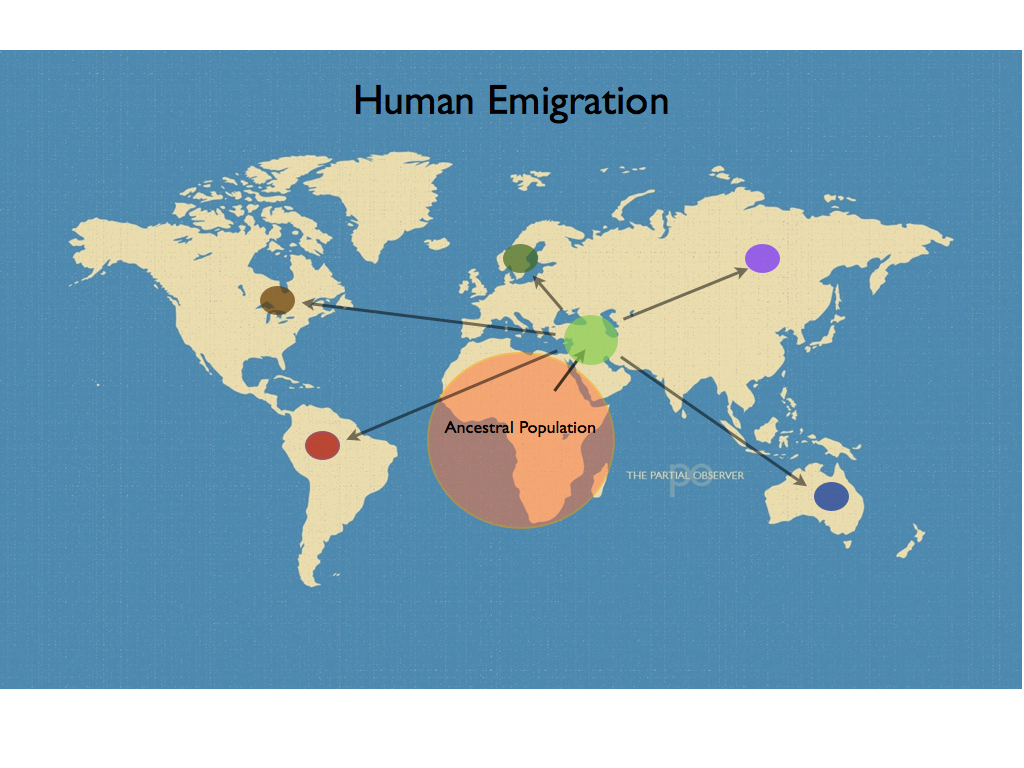
\includegraphics[width=0.9\textwidth]{../pictures/Single_origin_1.jpg}
	\caption{Human migration events: The picture describes how the populations have spread out from Africa about 125000-65000 years ago \cite{born_in_africa}. Circles represent the genetic diversity found in the populations.}
	\label{fig:human_migrations}
\end{figure}

\vspace{10 mm}


The most well studied example of this is humans, here the Out Of Africa Theory was founded before genetic material was accessible. The theory was based on archeological findings from around the world and the idea is that all humans originate in Africa and then migrated to the rest of the world, as illustrated in figure \ref{fig:human_migrations}.
 
These finding have then been confirmed over and over again when studying the genetic material of human populations. Since humans is a relatively young species we tend to see, as in figure \ref{fig:human_migrations} and \ref{fig:single_origin}, that almost all variants from any population can be found in the ancestral population, which is the African population south of Sahara.


\begin{figure}[ht]
	\centering
		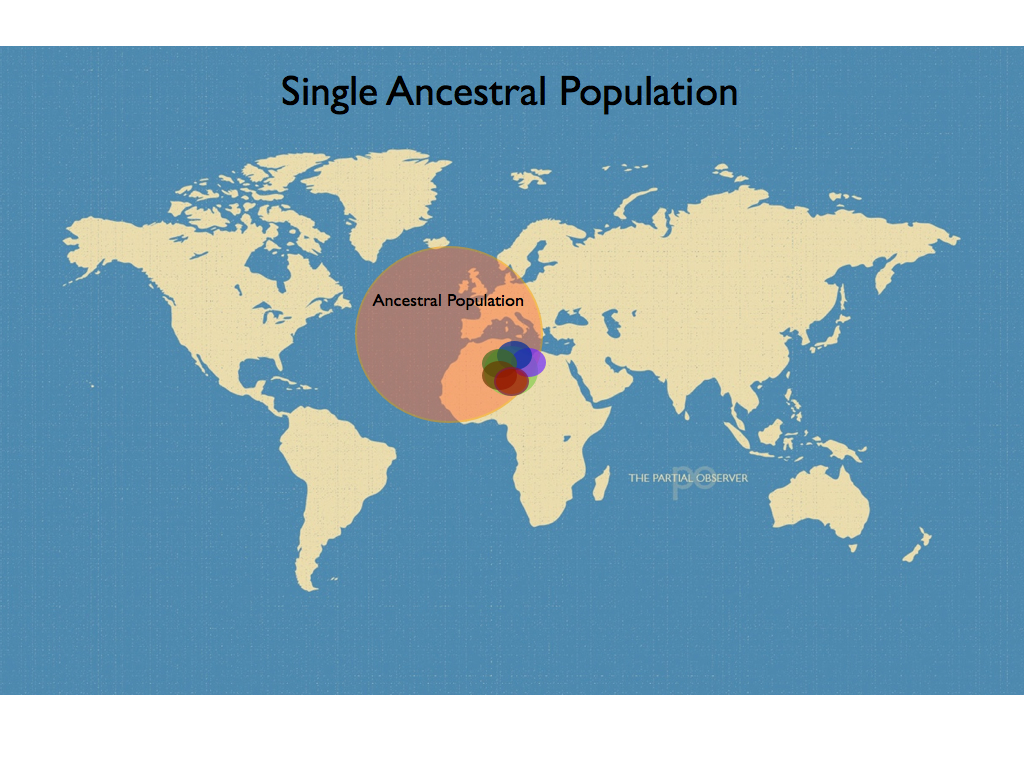
\includegraphics[width=0.9\textwidth]{../pictures/Single_origin_2.jpg}
	\caption{Human migration events: In the picture each circle represent the genetic diversity collected from populations all around the world. When compared to the suspected founder population, the African population south of Sahara here  represented by the the big circle, we find that all genetic variations from the populations can be found in the founder population.}
	\label{fig:single_origin}
\end{figure}

\vspace{3 mm}


% Kolla upp Y-chromosome som markör, kanske ska vara "en del y-kromosomen" av denna eller liknande.

When trying to infer population history from molecular data one has until recently been limited to using so called genetic markers. This means that a fairly small and easy accessible part of genetic material is revealed in individuals from as many populations possible, this limitation was due to lack of technology and cost of sequencing. Two well used markers has been \textbf{mitochondrial DNA (mtDNA)} and parts of the \textbf{Y-chromosome}. mtDNA is a small chromosome apart from the nuclear DNA that we usually think of as the genome, some of the advantages of mtDNA as a genetic marker is that they are abundant in cells and inherited only on the \textbf{maternal} side, they only recombinate with other almost identical mtDNA resulting in minimal structural variation and has a high mutation rate \cite{cann87}.
 
The Y-chromosome is inherited only on the \textbf{paternal} side and does also not recombine (except for a small part that recombines with the X-chromosome) \cite{underhill07}. The Y-chromosome has been examined in several human \cite{jobling03,kayser01} and animal population studies \cite{ginja08,ling10}. The more genetic markers that are used the more information we can get of the history of evolution. When studying a single genetic marker only, we can more or less get the big picture but if we want to know more specific things like time for bottleneck events, migration and so on we need to have more markers or, most preferable, whole genome data \cite{stoneking11}.

\section{Origin of Dogs}

Morphological, behavioral and molecular data all agree that dogs originates from wolf \cite{clutton-brock95,vila97,wayne93} but the geographical origin of dogs is still debated. The first ideas of origin are based on archeological findings that point to multiple breeding events in South West Asia and Europe\cite{clutton-brock95,dayan94}.

There are several problems with making assumptions from archeological data. Among others there will be bias to where the most excavations have been located. It can be hard to make a difference between species, in our case dogs and wolves, when there is only a limited amount of material.

The archeological findings haved been complemented with genetic information, and the ruling hypotheses are currently that dogs originate from either single or multiple wolf populations in Europe \cite{benecke87,verginelli05}, Middle East \cite{gray10,vonholdt10} and/or South East Asia \cite{savo02, pang09, ding11}.

In contrast to what figure \ref{fig:human_migrations} and \ref{fig:single_origin} show, if we had multiple origins and collected genetic informaton from different populations we would expect to see something like in figure \ref{fig:multiple_origin} and \ref{fig:no_common_variation}.

\begin{figure}[ht]
	\centering
		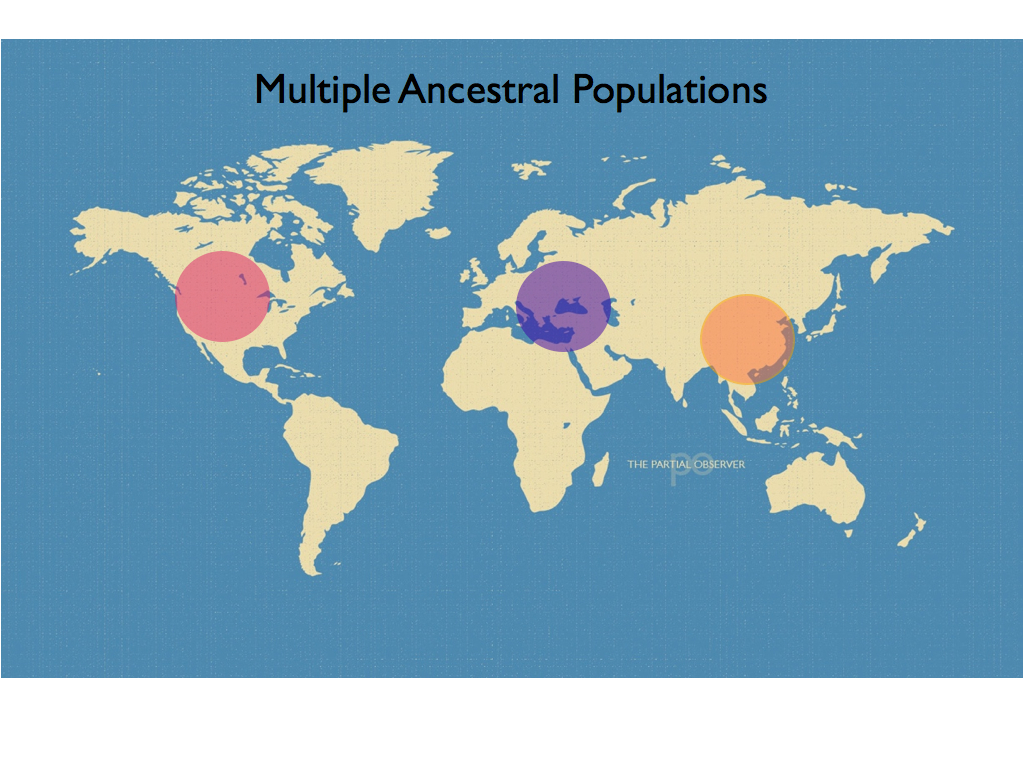
\includegraphics[width=0.7\textwidth]{../pictures/Multiple_ancestors_1.jpg}
	\caption{Multiple Ancestral Populations: The circles represent genetic pools of different populations.}
	\label{fig:multiple_origin}
\end{figure}

\vspace{3 mm}


\begin{figure}[ht]
	\centering
		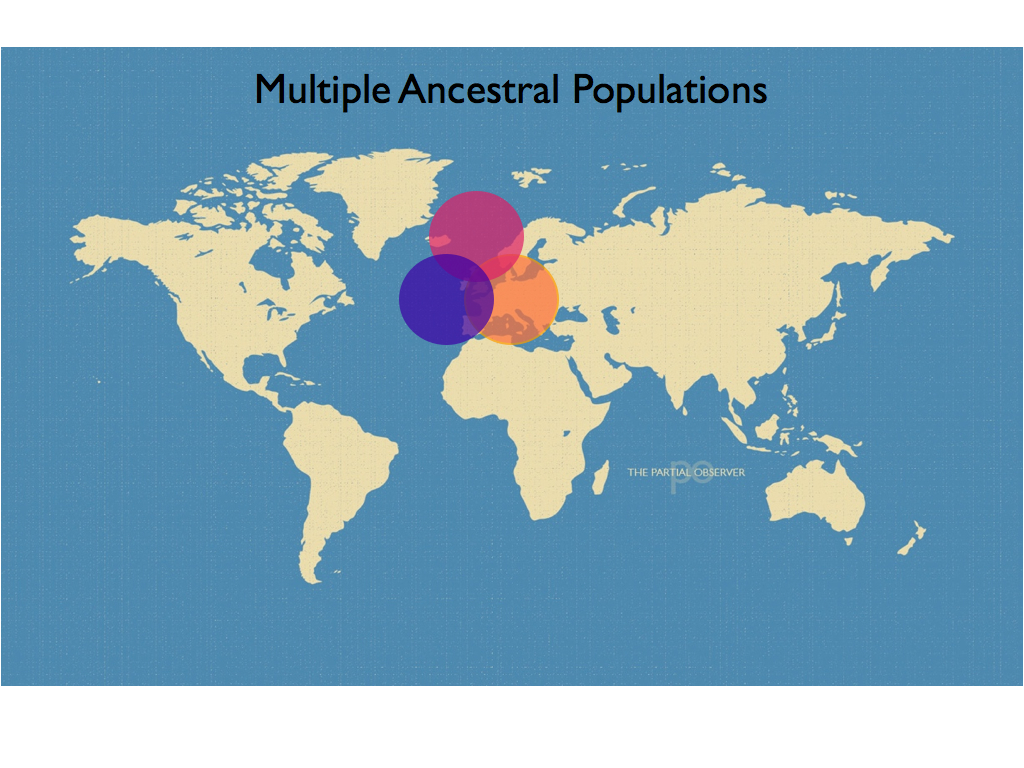
\includegraphics[width=0.7\textwidth]{../pictures/Multiple_ancestors_2.jpg}
	\caption{Multiple Ancestral Populations: If we where to compare the genetic information for populations of a species with multiple origin, we would expect to find large variations between the populations.}
	\label{fig:no_common_variation}
\end{figure}

\vspace{6 mm}


After looking at genetic variation in a small number of dog breeds for a forensic study, Peter Savolainen and co workers started to suspect a different view of dog origin \cite{savo97}. They could see that, even in a small data set, dogs from the asian breeds had a greater genetic diversity than dogs from other breeds.

In 2002, Savolainen et.{ }al.{ }published an article \cite{savo02} where they proposed a single East Asian origin for the domestic dog about 15,000 years ago, based on variation in parts of mtDNA. In a more extensive mtDNA study published 2009 \cite{pang09} 10 major haplogroups where found in dog populations from all around the world. Among these the only population to include all haplogroups was in South East Asia south of Yangtze River, implying a single origin in this region. The results where confirmed again in 2011 \cite{ding11} when variation in the Y-chromosome was studied.
These findings might seem unquestionable but there is still an ongoing discussion of how many times and where dogs where domesticated.
 
In this work we have tried to develop a method to genotype a small hypervariable region of genomic DNA with errors created during the sequencing process. If we succeed in genotyping these individuals, we can see how genetic diversity of this marker correlate with the earlier findings described above. We expect to see the biggest diversity among the wolves and the second biggest among dogs sampled south of Yangtze River.  


\chapter{Sequencing of a multivariable region and the problems that arise}

In the previous section we talked about population genetics and showed some attempts to pinpoint the location of origin of a species. We showed that a number of studies on a large set of dogs leads to a single origin in South East Asia, but the hypothesis is not fully recognized by the scientific community. In this section we will describe how another experiment was perfomed, where a new genetic marker is studied in the same dataset as before.

\section{Sequencing process}

A 270 bp long exon of the gene DLA-DRB1 was sequenced in 3461 dogs. DLA-DRB1 was choosen for beeing the most variable part of mammalian genomes, and is therefore an excellent marker for population genetic studies(see earlier section). Genetic material was extracted and enriched in about 40 PCR cycles and then prepared for sequencing by using a new technique described in \cite{neiman11} where a two tagging system made it possible to sequence up to 4992 samples in a single run. 

The actual sequencing was made using the 454 GS FLX Titanium Chemistry \cite{454_tech}, because of the length of the output reads from the 454 instrument. The perhaps more accurate Illumina instrument had a read length maximum of 100 high quality bases \cite{NextGen} at the time of the experiment, while the 454 instrument could produce read lengths of up to \textbf{500} bases \cite{454_problems}. With that length the whole exon of interest would fit in a single read, including primers. The most significant drawback of the 454 instrument is its problem with insertions and deletions, especially in homopolymeric regions \cite{454_problems}. We will show how this manifests in our data later.

Amplification of reads is a preparation that is necessary for all of the well used Massive Parallell Sequencing ({MPS}) instruments \cite{NextGen} and it is common that the {PCR} method \cite{pcr} is used. In short the sequence is extracted from the {DNA} in each individual and then labeled with two short tags for future identification. The two tagging system include one tag for the individual id and one for the plate id that the sequence is prepared on. After amplification the sequences are mixed, or pooled, and ready for sequencing. The sequence instrument has a maximum capacity of the number of reads that can be made in a run. These reads will be shared among the samples depending on how much sequence is available after amplification, with the result that some sample will get zero or very few reads and some samples will get a high coverage.

\section{Data}

Our data set consisted of a fasta file for each individual with between 20 and 425 reads. Data for individuals with fever reads was discarded since it was considered weak to draw any conclusion about the correct alleles. One read here means the 270 bp long exon with primer sequences, or tags, attached to both sides. The tags are known sequences with a length of 15 bp each. 

Moreover we had access to 113 published and soon to be published sequences (sequenced inhouse in an earlier project) of the same exon. These sequences had been validated by sanger sequencing \cite{sanger} and can be viewed as \emph{true} sequences, we'll call these \emph{reference sequences}.

Dog and wolf are, just like humans, diploid species which means that they have two copies of the genome in each cell, so if an individual have the same allele in both copies we say that this individual is \textbf{homozygote} for position \textbf{x}, and if there are two different alleles on the two copies we say that the individual is \textbf{heterozygote} in this position. A collection of alleles is called a \textbf{haplotype} and one can be homozygote or heterozygote for a haplotype. In a diploid species there are not more than two alleles of a region, but in a population there can be many alleles.

\section{A closer look at the problems}

If there where no errors during the enrichment and sequencing process the data for one individual would consist of a number of identical sequences, if the individual was homozygote for the loci.

If the individual is a heterozygote we could expect a distribution where about half of the reads where identical to one variant and the rest to the other, as in figure \ref{fig:perfect_heterozygote}.

\begin{figure}[ht]
	\centering
		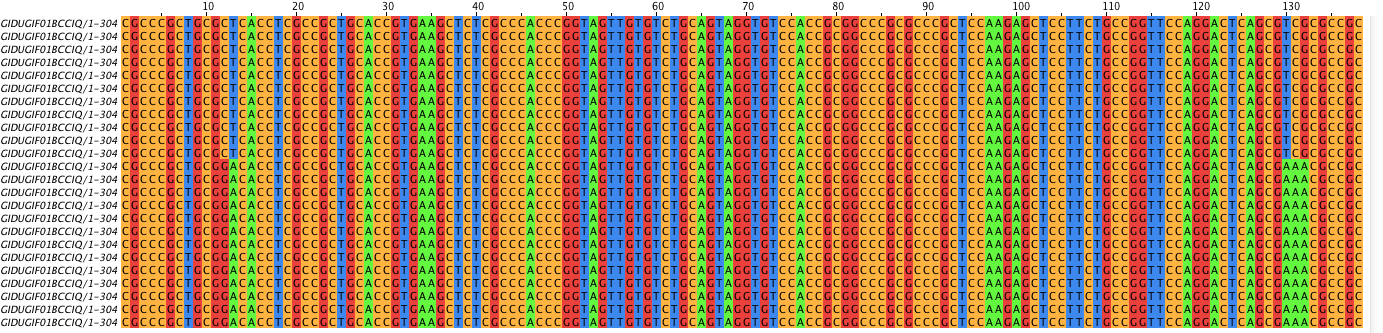
\includegraphics[width=\textwidth]{../pictures/../pictures/perfect_heterozygote.png}
	\caption{Ideal Heterozygote: In this picture we can see that the 11 first reads show the sequence of one of the alleles, and the last 13 from the other. There is no ambiguities in the data, that is why we call it a perfect heterozygote. (Figure does not show the full length of the sequence.)}
	\label{fig:perfect_heterozygote}
\end{figure}

\vspace{5 mm}


When the data is presented from the sequencer, many errors has arisen during the way, an example of real data can be seen in figure \ref{fig:align_chaos}.

\begin{figure}[ht]
	\centering
		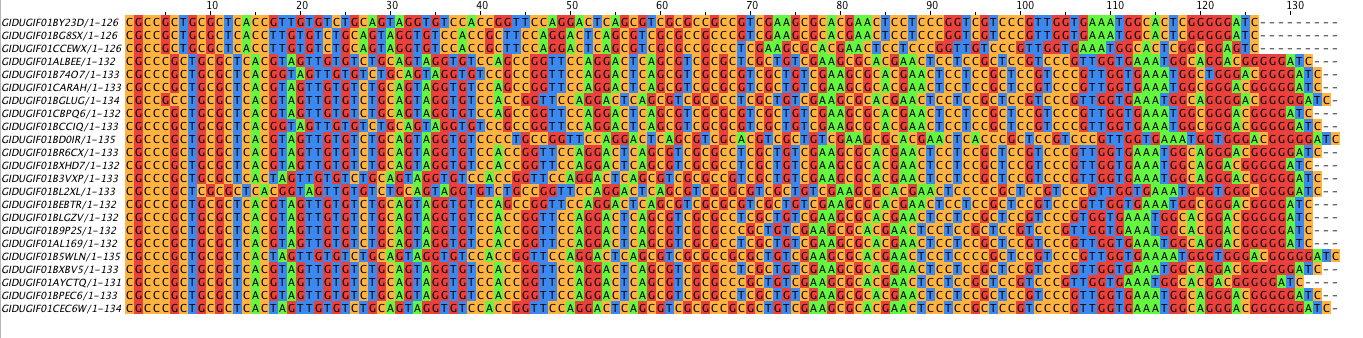
\includegraphics[width=\textwidth]{../pictures/align_chaos_cropped.png}
	\caption{Actual Data: This is an example of how the true data looks like for a heterozygote dog. The lengths of the sequences varies as a result of the 454 instrument problems with homopolymeric regions \cite{454_problems}. (Figure does not show the full length of the sequence.)}
	\label{fig:align_chaos}
\end{figure}

\vspace{5 mm}


We will now have a closer look at the different problems that can explain why figure \ref{fig:perfect_heterozygote} and figure \ref{fig:align_chaos} differ som much. To illustrate them we use a simplified figure, like figure \ref{fig:true_alleles}.

\begin{figure}[ht]
	\centering
		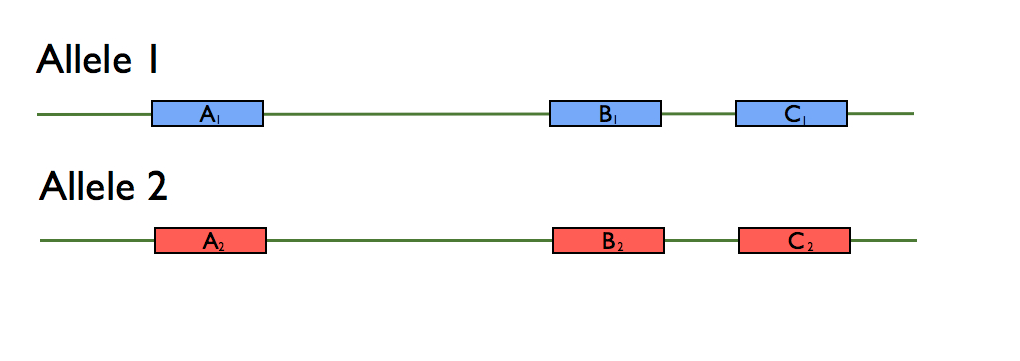
\includegraphics[width=0.9\textwidth]{../pictures/True_Alleles.png}
	\caption{Simplified sequence: This is a picture where we have collapsed the parts that are identical between the alleles, boxes represent positions where the alleles differ and the colours mark different variants.}
	\label{fig:true_alleles}
\end{figure}


\begin{itemize}
	\item \textbf{Single nucleotide variations}
	This is the case where the reads do not share the same base in a certain position. These variations can be true heterozygote variations or machine errors. If we trust that our alignment is correct this problem can be handled fairly simple since a true variation should be found in about half of the reads, like in figure \ref{fig:true_snv}. A read error is expected to be a random event and would therefore only be seen in a few number of reads as seen in figure \ref{fig:false_snv}.

	\begin{figure}[ht]
		\centering
			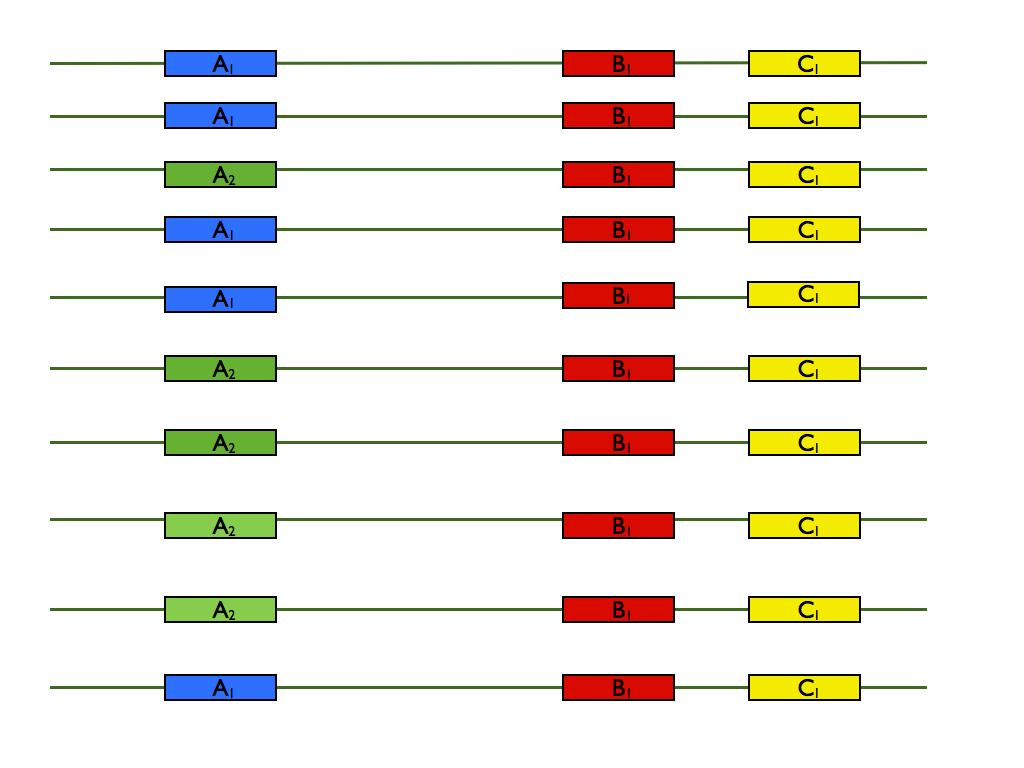
\includegraphics[width=0.7\textwidth]{../pictures/True_SNV.jpg}
		\caption{Expected pattern of a true SNV in simplified form, the variation appears in several reads.}
		\label{fig:true_snv}
	\end{figure}
	
	\begin{figure}[ht]
		\centering
			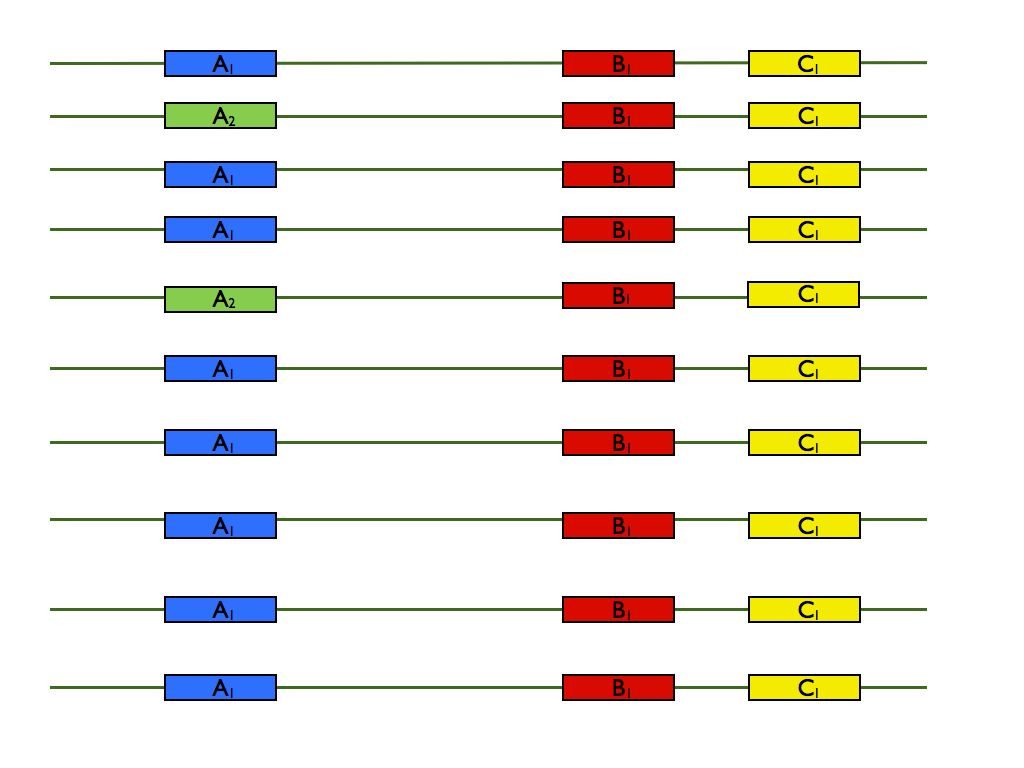
\includegraphics[width=0.7\textwidth]{../pictures/False_SNV.jpg}
		\caption{Expected pattern of a read error, the variation is rare or unique.}
		\label{fig:false_snv}
	\end{figure}
	
	\item \textbf{Insertion and deletions}
	Natural insertions or deletions (indels) in our sequence are highly unlikely. If the size of an indel is not a multiple of 3 it will cause a \emph{frameshift}. This means that the whole sequence of amino acids that the region is coding for after the indel will get displaced. A frameshift would most probably be lethal when occuring in such a vital part of the genome as this and combined with the fact that frameshift/nonframeshift indels in this region have not been observed in any of the published sequences we are not suspecting them to be true if observed in our data.
	
The 454 instrument will, especially in homopolymeric regions, make false insertions and/or deletions, this is a well known drawback of this technology \cite{454_problems}. As an example of this problem we observed in our dataset that a conserved part of the sequence has a homopolymer with 5 consecutive C:s. We found that, out of all reads, 0.03 \% had one C, 0.1 \% two C:s, 30 \% three, 56 \% four and only 13 \% showed all five C:s.	It might be true deletions but in this case it seems highly unlikely since all earlier observed reference sequences had 5 C:s in these positions.
	  
	\item \textbf{Chimeric sequences}
	Chimeric sequences can be thought of as artificial recombination and is formed during PCR amplification. When two segments from different {DNA} molecules are partially copied and added together, they give rise to false sequences that are very similar to the true alleles, example shown in figure \ref{fig:chimeric_sequences}.
	
If a chimer is created in the early steps of the PCR they will show up in a large number of the reads for the individual, these are hard to handle. Our data was expected to include many chimeric sequences as a consequence of the large number of PCR cycles that was performed. This has been the hardest problem to handle of the ones mentioned.

% Distinguish from real new alleles

\end{itemize}

\begin{figure}[ht]
	\centering
		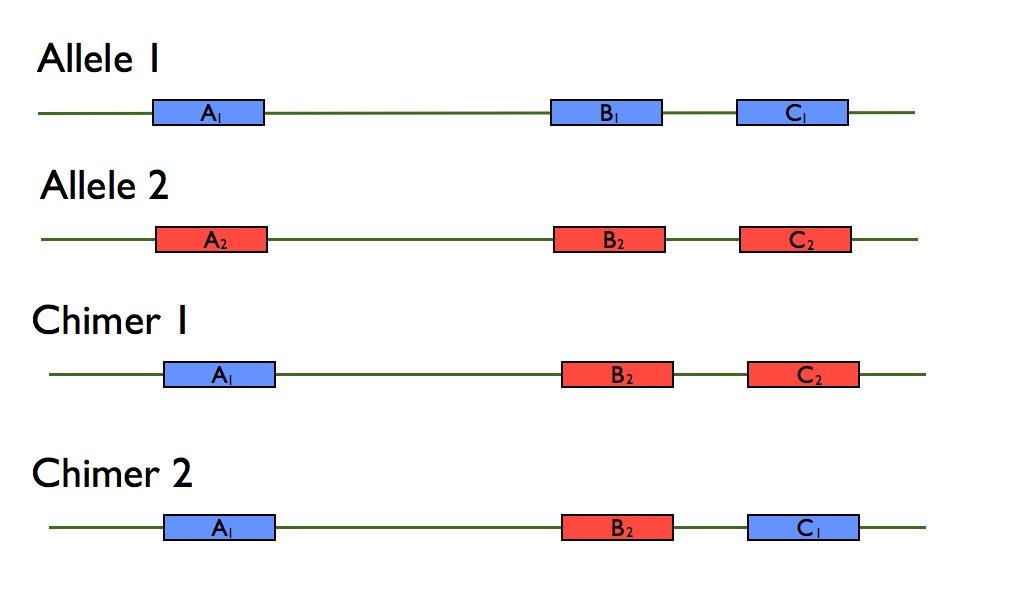
\includegraphics[width=0.7\textwidth]{../pictures/Chimers.jpg}
		\caption{Chimeric Sequences: The first two figures illustrates two alleles. Next we get two examples of how chimeric formations might look when segments from the true alleles, that include variations, have been partially copied and annealed together.}
	\label{fig:chimeric_sequences}
\end{figure}


Since there are machine artifacts in the form of indels and read errors the first thing one would like to do is to align the reads so that they will be comparable, then we might be able to detect what is true variations and what is sequencing/PCR errors. In the next section we will see what methods we used to find the true sequences in our data.




\chapter{Method}

As a consequence of the errors described in the previous section, there is such a variance in the sequences that we can not expect to see a true allele in any one of the reads of an individual. A first step to attack this problem is to make an alignment of all the sequences of a individual in such a way that each nucleotide end up in its correct position of the 270 base pair long sequence. This implies that we need to identify where in the sequences there is missing data, that is a machine induced deletion, and where the machine have made false insertions. A satisfying result could look like in figure \ref{fig:dream_scenario}.

\begin{figure}[ht]
	\centering
		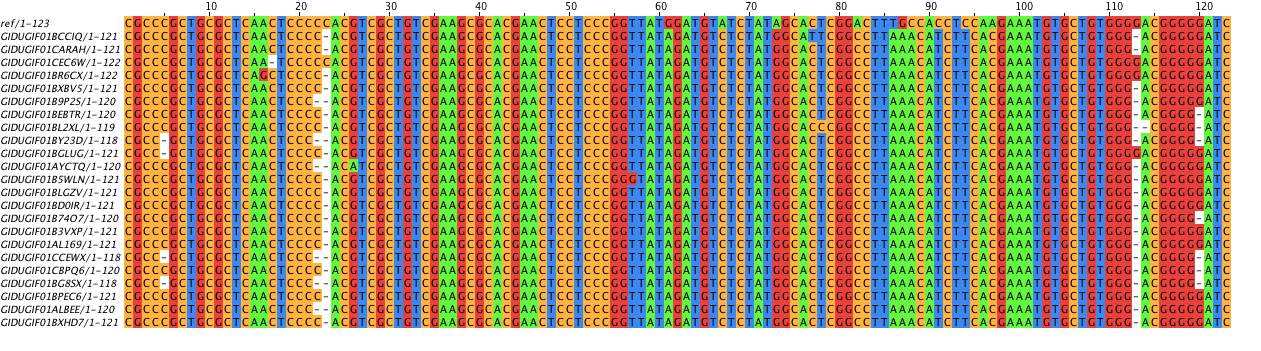
\includegraphics[width=\textwidth]{../pictures/align_with_ref_cropped.png}
	\caption{Aligned sequences. Picture does not show the full sequence.}
	\label{fig:dream_scenario}
\end{figure}


When the alignment is done we need to figure out what parts of the sequences that holds information about the true alleles and what parts that are chimeric formations or machine errors. The problem can be divided into two main parts with two separate methods to handle them. We start this section with an overview of the workflow, the steps are described in more detail in the following section:

\begin{enumerate}
	\item \textbf{Align the reads}
	\item \textbf{Identify the alleles}
\end{enumerate}

\section{Process Overview}

\begin{itemize}
	\item \textbf{Alignment} \\
	
	\textbf{Data in:} One file in fasta format for each of the individuals with raw sequence data.\\
	\textbf{Data out:} One file in fasta format for each of the individuals aligned sequences.\\
	
	% Indata Utdata
	
	\begin{enumerate}
		\item \textbf{Add tags}\\ 
		\textbf{for each} reference sequence:\\
		Add the same tags that were used for sequencing, these are present in all of our data but not in the references.
		\item \textbf{Build reference profile}\\
		\textbf{for all} reference sequences:\\
		Look at the frequency of \emph{A,C,G,T} in every position to estimate the scores for each bases in each position.
		The result is a unique scoring scheme for each position that we call a Reference Profile.
		\item \textbf{Align the sequences}\\
		\textbf{for each} sequence in each individual:\\
		Align the sequences globally, pairwise with the most abundant reference sequence (known as 00101) using the reference profile.
	\end{enumerate}
	\item \textbf{Choose Alleles} \\ 
	
	\textbf{Data in:} One file in fasta format for each of the individuals with aligned sequences.\\
	\textbf{Data out:} A fasta formatted file with one or two alleles for each individual.\\
	
	\begin{enumerate}
		\item \textbf{Find the variable positions}\\
		\textbf{for each} individual:\\
		Find out what are true differences and what is errors among the reads of an individual.
		\item \textbf{Start building the alleles}\\
		\textbf{for each} individual:\\
		Walk trough each position in the sequence and add it to the two alleles. If there is a variation in a position, find out which variation belongs to which allele and add them to the correct one. 
		\item \textbf{Compare with reference}\\
		\textbf{for each} allele:\\
		Compare the alleles to all reference sequences pairwise to see which of the references that is most similar.
		\item \textbf{Complete the alleles}\\
		\textbf{for each} allele in each individual:\\
		Fill the deletions with the corresponding base from the most similar reference sequence.
		\item \textbf{Remove tags}\\
		\textbf{for each} sequence in each individual:\\
		We can now safely remove the tags by chopping of the ends of the alleles.
	\end{enumerate}	
\end{itemize}



\section{Alignment}

At first glance one might think that the best and least biased way of getting order to the reads would be to multialign them for each individual. This problem is fairly hard and we tried a number of well known software like MAFFT \cite{mafft} , Muscle \cite{muscle} and Mosaik \cite{mosaik} but none of the models was suitable for our data. In general these softwares could not handle the problem with indels we had in our data.

From the nature of the DLA region one can assume that some parts of the sequence are highly conserved and thereby probably crucial for the function of the protein product. While other parts of the sequence are very variable which seems to be favourable for detecting foreign substances. As discussed in the previous section we will not allow any frameshift insertions or deletions in this exon since it is probably fatal for the product. We want an algorithm that takes advantage of this knowledge in such a way that when, for example, there is a homopolymeric region it is more favourable to do deletions in the end of the homopolymer than in the beginning, since we have observed that almost all homopolymers of length greater than 3 are too short in our data.

Our tool of choise was a dynamic programming algorithm for pairwise global sequence alignment, presented by \emph{Saul B. Needleman} and \emph{Christian D. Wunch} \cite{nw} in the early 1970:s. To use global alignment seems natural here when the sequences are very similar and we assume that they should all be of the same length.

The modifications we did was to make a scoring table with a unique scoring scheeme for each position in the reference, this could be done because we had acces to a fairly large number of reference sequences to base the table on. We call this our \emph{Reference Profile.}\\

% In the origninal version of Needleman-Wunch one uses a score matrix with penalties for the diferent matching types, finally the alignment with the lowest score is the optimal alignment. In our version we have swapped the numbers so if a match is more likely it gets a higher score and the optimal alignment is the one with the highest score. It does not really matter which way one does it, we thought it was easier to think of the problem this way.\\

% Skriv ut målfunktionen

\begin{enumerate}

	\item \textbf{Add the same tags to references that was added to all individuals}

Since the tags used for identification have been sequenced in the same way as the rest of the region they will also have the same problems with indels and error when reading bases, so it is not a trivial problem to remove the tags (we can not just remove a certain length of each end, or use a regular expression to find a pattern to remove). But it is a trivial task to add them to the reference sequences since we know the exact sequence of the tags (they are constructed). We believe that our alignment algorithm, given a reference sequence and a scoring table, can make a correct alignment, so the easiest way to remove the primers is to first align them and then remove them.

	\item \textbf{Creating the reference profile}

The sequence we want to use in our alignment is called a reference profile since each position have a distribution between a number of alternative nucleotides instead of a static score matrix that is identical for every position. The positions where all reference sequences agree on the same nucleotide are used as `anchors'. We assume that these positions are conserved and therefore we can almost force the algorithm to align correctly against them and be more `loose' in the variable and homopolymeric parts of the sequence.

We base our scoring scheme on the frequencies of the nucleotides in each position from the set of reference sequences. Each position also got a fixed negative score for insertion, represented by a gap in the reference sequence, and a fixed negative score for deletion, represented by a gap in the sequence to align. These scores are negative because the indels made by the machine is almost only happening in homopolymers so we do not want to see them in our alignment anywhere else, but they are still allowed.

As mentioned earlier, the instrument have problems with homopolymeric sequences and almost allways show to few bases when reading these. To correct for this error we give a positive score for deletions that increases with the length of the homopolymer. This scoring is done in a heuristic fashion based on our observations.

\vspace{10 mm}

	\item \textbf{Make a pairwise global sequence alignment with the most abundant reference}

In short, the algorithm walks trough the two sequences and evaluates every possible pair by using a table with different scores for match, mismatch, insertion and deletion. The alignment with the highest score is the optimal alignment with the given score matrix. After alignment we remove all sites where there are gaps in the reference sequence. If our alignment is correct these represents insertions in the sequence to align and according to the asumption made above they are not allowed. No sequence is now longer than the reference sequence but almost all are shorter as a consequence of the deletions from the sequence instrument. Figure \ref{fig:aligned_sequences} show how an aligment of the sequences would look like.

\begin{figure}[ht]
	\centering
		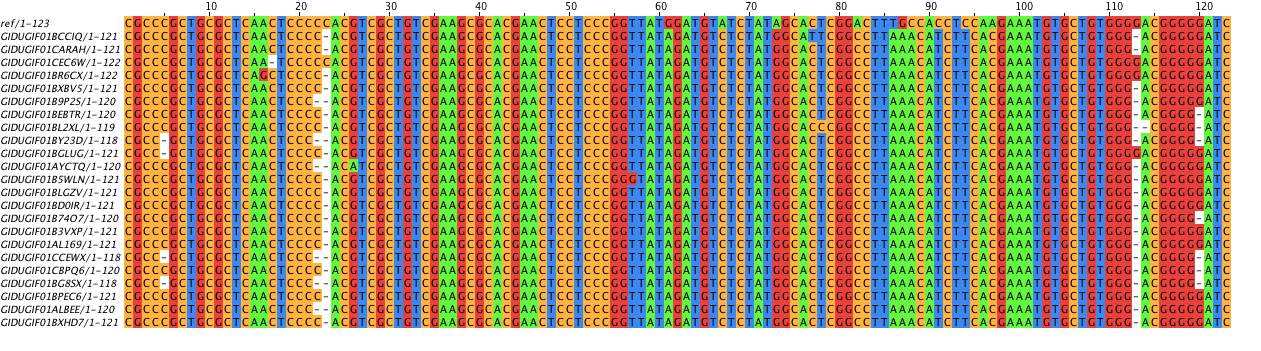
\includegraphics[width=\textwidth]{../pictures/align_with_ref_cropped.png}
	\caption{Aligned sequences with the reference in top.}
	\label{fig:aligned_sequences}
\end{figure}

\end{enumerate}



\section{Choose Alleles}

\begin{figure}[ht]
	\centering
		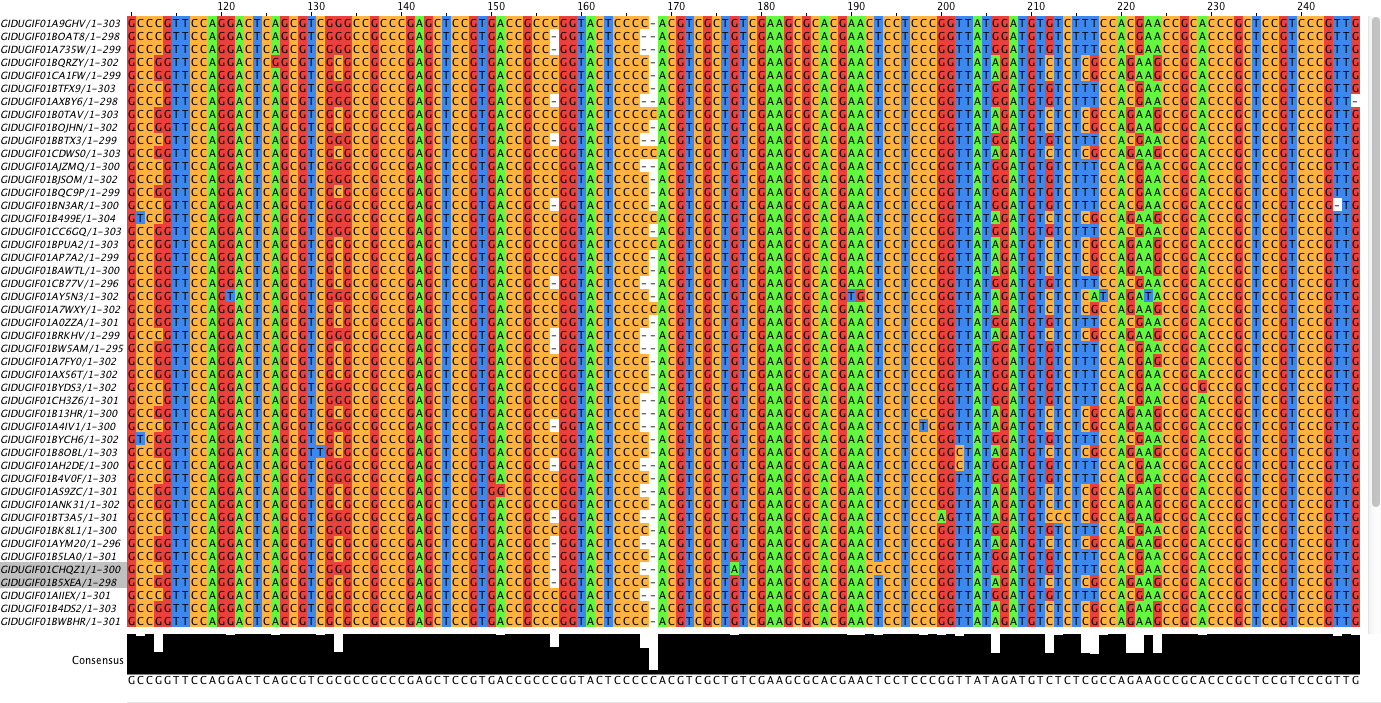
\includegraphics[width=\textwidth]{../pictures/align_example.png}
	\caption{Aligned sequences}
	\label{fig:many_aligned_sequences}
\end{figure}


We can think of the alignment like in figure \ref{fig:many_aligned_sequences}, that all sequences are put on top of each other like rows in a matrix, then each column in the matrix represents a position in the sequence. The differences between two alleles are of course the differences in certain positions of the sequence, the rest will be identical. But as we can see, there are some noice in the form of read errors that needs to be distinguished from true variation. Most of these columns will have more or less the same nucleotide in all rows but in some cases there will be a distribution between two or more bases, in the \emph{true} sequences we do not allow more than two variants in one position since this would imply more than two alleles. If there is enough variation in a position for us to believe that is true and not an error we call this position a \emph{variable position}.

If there is no variable positions among the sequences the individual is a \emph{homozygote}, if there are at least one variable position the individual is a \emph{heterozygote}. The problem here is to determine if a variation is real or created during sequencing. 

\begin{enumerate}
	\item \textbf{Count the frequencies for each position}

	For each position of the exon, which is represented by a column in our aligned matrix, we look at the distribution over the nucleotides or insertions. The original sequence is 270 base pairs long, but as a consequence of insertions and deletions the length might vary. We call the positions $n$ and the frequencies $q_a$ where $a\in \{A,C,G,T,-\}$. So each position $n$ has a distribution like $d_n: \lbrack q_A=x_1, q_C=x_2, q_G=x_3, q_T=x_4, q_{-}=x_5 \rbrack $ and $\sum_{i=1}^{5}x_i = 1$.
	
We call the frequency of the most abundant variation in position $n \, q_n^1$, the second most abundant $q_n^2$ and so on, these frequencies represents a nucleotide. Then if $q_n^2 = 0 \implies q_n^1=1$, and both alleles have the same nucleotides in position $n$, and if $q_n^1 = 1, \, \forall \, n \implies$ homozygous individual.

	\item \textbf{Choose a treshold for variable positions}

	We have to decide \emph{when} we say that a position is variable since this will determine if an individual is hetero- or homozygote and for which positions the sequences differs. If $q_n^2$ is very small we might assume that the distribution is a consequence of some kind of error in the process. We want to find a treshold that is reasonable, if we for example set the threshold such that if the second most abundant nucleotide is in 10 \% of the reads we call it a variable position(implying a heterozygote), this will mean that an individual with 20 reads needs the same variation in only 2 of them to give rise to a second allele, this might be accomplished by read errors so we need to be a bit careful. In the figure \ref{fig:het_hom_relation} we can see how the relation between hetero- and homozygote individuals varies when changing this treshold for $q_n^2$.

	\begin{figure}[ht]
		\centering
			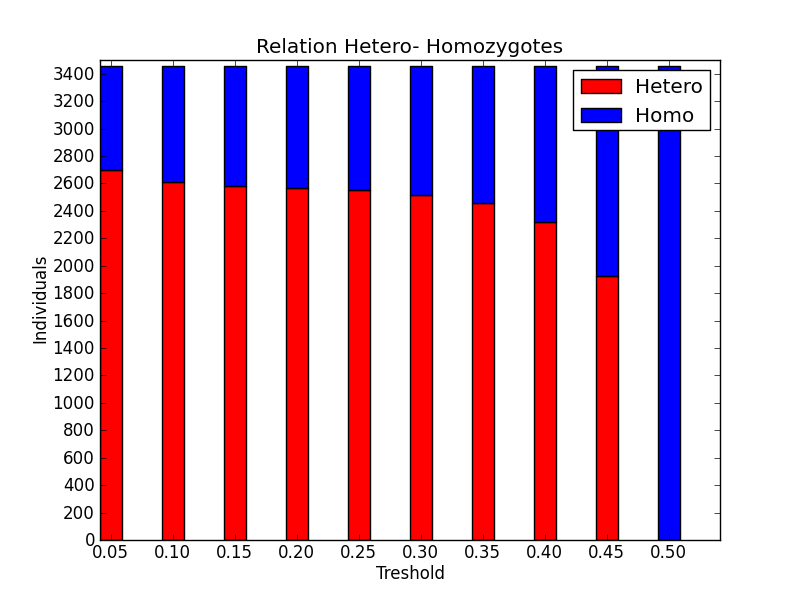
\includegraphics[width=0.9\textwidth]{../pictures/het_hom.png}
		\caption{Relation between hetero and homozygotes when $q_n^2 < treshold$. It is enough with a single variable position to count the individual as a heterozygote.}
		\label{fig:het_hom_relation}
	\end{figure}


	There are many errors in our data and we need to be careful of creating novel sequences with these errors. We prefer to miss some alleles (e.g. say that an individual is homozygote when they are heterozygote) in a few individuals rather than to report false sequences. We chose the Variable Position Treshold ($VPT$) such that the second most abundant nucleotide must be present in at least 35 \% of the reads to qualify as a variable position.

	\item \textbf{Build the alleles}

	To produce the alleles we walk through the sequence, starting from position 1 and look at $q_1^2$. If $q_n^2 \leq \, VPT$ we add the nucleotide represented by $q_n^1$ to position $n$ in both allele sequences $A^1$ and $A^2$. If $q_n^2 > \, VPT$ we have a variable position, $V_i$, so one variant should be added to both alleles at position $n$, we denote this as $A^1_n$ and $A^2_n$. If it is the first variable position, $V_1$ (notice that this is not the first position of the sequence, it is the first variable position for the sequences), it does not matter how we add the variant since both alleles are identical up till now. If the n:th position is a variable position $V_i, \, i \neq 1 $ we need to decide which variant should be added to which allele. One thing that makes the situation complicated is the chimeric formations of the sequences. Remember that they consist of segments of sequences that has been copied and annealed together to form new artificial sequences. Our method is based on the idea that the majority of the reads of an individual have the correct sequence if looked at in portions.
	
	So when we have a variable position $n = V_i, \, i \neq 1$, that is position $n$ which is also the variable position number $i$, we sort all sequences based on what variation they had in the previous variable position, $V_{i-1}$, into two groups $G^1$ and $G^2$. Each of these groups have a consensus nucleotide at every position $n$ that we call $G^j_n$. Since we sorted the sequences based on what nucleotide they had in position $V_{i-1}$ we know that $G^1_{V_{i-1}} \neq G^2_{V_{i-1}}$. We then compare $G^1_{V_{i-1}}$ to $A^1_{V_{i-1}}$ if they are the same we set the consenseus nucleotide $G^1_n$ to $A^1_n$ and $G^2_n$ to $A^2_n$. If $G^1_{V_{i-1}} \neq A^1_{V_{i-1}}$ we set $G^2_n$ to $A^1_n$ and $G^1_n$ to $A^2_n$.

	\item \textbf{Produce the final allelic sequences}

	There are now two alleles with almost identical sequences if the individual is heterozygote or two identical alleles if homozygote. Some problems are still left; there are positions where $q_n^1$ represents $-$, which means that the alleles have a deletion in position n, these has to be filled with something. To do this we want to find the most similar reference sequence and insert the corresponding variant here. The idea here is that all sequences have a relationship in the sense that they have evolved from the same original sequence. So the sequence that is most similar over the full length is most likely to have the same base in the unknown position in question. This is done by calculating the similarity between the allele and all of the reference sequences and then fill the gaps with the corresponding nucleotide from the most similar reference sequence.

	\item \textbf{Remove the tags}

	We assume that our algorithm made a perfect alignment so we can simply cut the beginning and end of each sequence to get the full exon only.


\end{enumerate}

\chapter{Results}


In the collection of \textbf{3461} dogs we found, with our method, that they had \textbf{366} variants or alleles of DLA-DRB1. There were \textbf{769} or \textbf{22 \%} homozygous individuals. \textbf{79} of the alleles had already been found in earlier genotyping projects so \textbf{287} are novel. Of the novel alleles \textbf{25} where found in homozygous individuals. \textbf{179} of the alleles where found in one individual, \textbf{34} in two and \textbf{28} in three individuals. Of the `known' alleles \textbf{35} where not found at all in this dataset. 

\begin{figure}[ht]
	\centering
		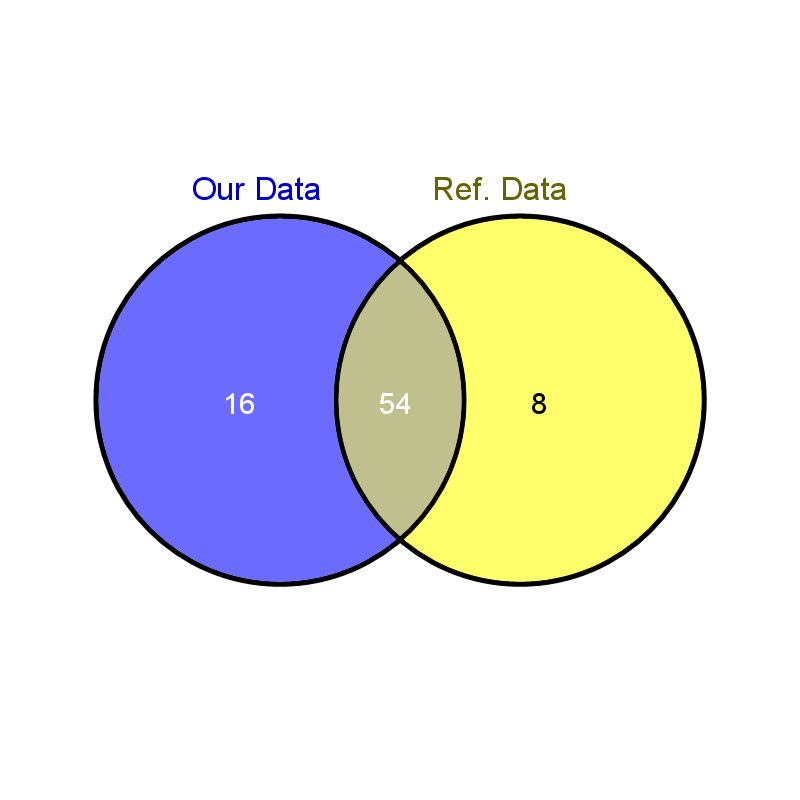
\includegraphics[width=0.9\textwidth]{../pictures/variants.png}
	\caption{Found variants contra reference variants: The figure shows how many variants that the reference sequences and our data set had in common.}
	\label{fig:variants}
\end{figure}

As seen in figure \ref{fig:variants}, \textbf{8} positions had variations that where unique for the reference sequences and \textbf{16} new positions with variation in our data set that have not been seen before. \textbf{54} positions of the \textbf{270} base pair long exon had variation in both the reference alleles and the genotyped dataset.


\section{Discussion and Conclusions}

When we started to investigate the data we discovered that it was fairly easy to make the alignments by hand. By looking at the sequences we could figure out where it most probably where machine errors contra true variations, or where it should be an insertion or a deletion. Chimeric formations are still hard to detect by eye in a sequence of this length. We tried to understand \emph{how} we could tell that the alignments produced by the named softwares are wrong. The conclusion is that we want to incorporate prior knowledge we had about this exon and the sequencing technology into the alignment algorithm, this was how our method was developed.

The best way to evaluate the results would have been to compare the variations between different breeds and regions. We would expect to see low variation of alleles within a pure breed, since these stem from a few individuals only. We would also expect to see a greater variation in mixed breeds and the highest diversity in wolves.

Unfortunately the geografic information for the samples are currently missing but if the individuals can be linked to their region of origin in a correct way, the results of this work can help to clarify the origin of dogs. Hopefully this would strengthen any of the hypotheses of dog origin by showing which population that show the highest variety of alleles.

It is reasonable to belive that some new variable positions is to be seen in a large set of data like this. There is a problem that many of the new alleles were only found in only one individual, it seems unlikely that we see this as often as we do. It is hard to tell how many of these alleles that are false positives based on numbers, but a guess from the initiator of this project was to find about 400 alleles all in all.

Personally i think that the alignment algorithm works fine and do not think that the problems can be traced to this part of the process. Several people have inspected the results of the alignment, and all agree that the algorithm produces the same result as we would have done by hand. The question is how close we can get to reality with such problematic data.



% \addcontentsline{toc}{section}{Appendix}


% \code{Sequences}{../code/sequences.py}
% \code{Fasta Parser}{../code/fasta_parser.py}
% \code{Add Tags}{../code/add_tags.py}
% \code{Check Homopolymers}{../code/check_homopolymers.py}
% \code{Check Homozygotes}{../code/check_homozygotes.py}
% \code{Check Alleles}{../code/checkAlleles.py}
% \code{Fill Sequence}{../code/fill_sequence.py}
% \code{Needleman Wunch}{../code/NW.py}
% \code{Parse Individual}{../code/parse_individuals.py}
% \code{Plot Hetero- and Homozygotes}{../code/plot_het_hom.py}
% 

% \appendix

\appendix
\renewcommand\thechapter{}
\renewcommand\thesection{\arabic{section}}
\chapter{Code}


Code is available at \url{https://github.com/moonso/DLA_Genotyper}


% \begin{figure}[ht]
% 
% \begin{center}
% And here is a figure
% \caption{\small{Several statements describing the same resource.}}\label{RDF_4}
% \end{center}
% \end{figure}
% 
% that we refer to here: \ref{RDF_4}
\bibliography{mybib}{}
\bibliographystyle{plain}

\end{document}
